\chapter{Memorias Digitales}

\section{¿Qué es una memoria?}

La memoria es la parte de un sistema digital que almacena datos binarios en grandes cantidades. Está formada por matrices de elementos de almacenamiento ---biestables o capacitores--- capaces de retener un bit de información cada uno.

En un sistema microprogramable la memoria cumple dos funciones distintas:

\begin{itemize}
  \item \textbf{Memoria de programa:} almacena las instrucciones que la CPU va a ejecutar. No se modifica durante la ejecución del programa. Se implementa en memoria no volátil (Flash, ROM).
  \item \textbf{Memoria de datos:} almacena las variables y resultados intermedios del programa. Se modifica constantemente durante la ejecución. Se implementa en RAM (volátil).
\end{itemize}

\section{Unidades de datos binarios}

\begin{table}[H]
\centering
\begin{tabular}{llp{7cm}}
\toprule
Unidad & Tamaño & Descripción \\
\midrule
Bit & 1 bit & Unidad mínima de información: un 0 o un 1 \\
Nibble & 4 bits & Medio byte; útil en representación BCD \\
Byte & 8 bits & Unidad básica de almacenamiento en la mayoría de los sistemas \\
Palabra (\textit{word}) & variable & Unidad completa de trabajo de la CPU (8, 16, 32 o 64 bits según la arquitectura) \\
\bottomrule
\end{tabular}
\end{table}

Las capacidades de memoria se expresan en múltiplos de byte:

\begin{table}[H]
\centering
\begin{tabular}{ll}
\toprule
Múltiplo & Equivale a \\
\midrule
1 Kbyte (KB) & $2^{10}$ bytes = 1.024 bytes \\
1 Megabyte (MB) & $2^{20}$ bytes = 1.048.576 bytes \\
1 Gigabyte (GB) & $2^{30}$ bytes = 1.073.741.824 bytes \\
\bottomrule
\end{tabular}
\end{table}

\section{Organización interna: la matriz de memoria}

Internamente, una memoria se organiza como una \textbf{matriz de celdas}, donde cada celda almacena un bit. La forma en que se agrupan esas celdas determina la organización de la memoria.

\tikzFigura{cap2/matriz-organizaciones}{Una misma matriz de 64 celdas organizada como 64$\times$1, 8$\times$8 y 16$\times$4. Cada fila es una palabra (resaltada).}

Por ejemplo, una matriz de 64 celdas puede organizarse como:

\begin{itemize}
  \item \textbf{64 $\times$ 1:} 64 palabras de 1 bit cada una.
  \item \textbf{8 $\times$ 8:} 8 palabras de 8 bits (8 bytes).
  \item \textbf{16 $\times$ 4:} 16 palabras de 4 bits (16 nibbles).
\end{itemize}

La \textbf{capacidad} de una memoria se calcula como:

$$\text{Capacidad} = N_{\text{direcciones}} \times \text{longitud de palabra}$$

\textbf{Ejemplos:}

\begin{itemize}
  \item Una memoria 16 $\times$ 4: 16 posiciones $\times$ 4 bits = 64 bits en total.
  \item Una memoria 16K $\times$ 8: $16.384$ posiciones $\times$ 8 bits = 131.072 bits = 16 KB.
\end{itemize}

\begin{notabox}
Los números de posiciones son siempre potencias de 2. El ``16k'' es en realidad $2^{14} = 16.384$, redondeado a la unidad más próxima por convención.
\end{notabox}

\section{Direccionamiento}

Cada posición de la matriz tiene una \textbf{dirección}: un código binario único que la identifica. Para acceder a una posición se coloca su dirección en el \textbf{bus de direcciones}; un decodificador interno selecciona la fila y columna correspondientes.

\tikzFigura{cap2/memoria-buses}{Memoria 1K$\times$8: bus de direcciones (A0--A9), bus de datos bidireccional (D0--D7) y señales de control activas en bajo ($\overline{CS}$, $\overline{OE}$, $\overline{WE}$).}

La cantidad de posiciones direccionables depende del número de líneas del bus de direcciones:

$$N_{\text{posiciones}} = 2^{N_{\text{líneas de dirección}}}$$

\textbf{Ejemplo:} una memoria con 10 líneas de dirección (A0--A9) puede tener $2^{10} = 1.024$ posiciones.

\section{Operaciones básicas: lectura y escritura}

Para controlar si una operación es de lectura o escritura, y para habilitar o deshabilitar el chip, las memorias disponen de señales de control. Las más comunes son:

\begin{table}[H]
\centering
\begin{tabular}{llp{7cm}}
\toprule
Señal & Nombre & Función \\
\midrule
$\overline{CS}$ (o $\overline{CE}$) & \textit{Chip Select / Chip Enable} & Activa el chip (activa en bajo). Permite conectar varios chips al mismo bus y seleccionar solo uno a la vez \\
$\overline{OE}$ & \textit{Output Enable} & Habilita las salidas de datos durante una lectura \\
$\overline{WE}$ & \textit{Write Enable} & Habilita la escritura de datos \\
\bottomrule
\end{tabular}
\end{table}

\subsection{Operación de escritura}

\begin{enumerate}
  \item Se coloca la dirección en el bus de direcciones.
  \item Se activa $\overline{CS}$ (se pone en bajo).
  \item Se coloca el dato en el bus de datos.
  \item Se activa $\overline{WE}$ (pulso en bajo): el dato queda grabado en la posición seleccionada.
\end{enumerate}

\tikzFigura{cap2/escritura-timing}{Diagrama de tiempos de una escritura. Los números corresponden a los pasos del texto; el dato se graba en el flanco ascendente de $\overline{WE}$.}

\begin{advertenciabox}
Escribir en una posición \textbf{destruye} el dato que había antes en esa dirección.
\end{advertenciabox}

\subsection{Operación de lectura}

\begin{enumerate}
  \item Se coloca la dirección en el bus de direcciones.
  \item Se activa $\overline{CS}$ (se pone en bajo).
  \item Se activa $\overline{OE}$ (se pone en bajo): la memoria deposita el dato almacenado en esa dirección sobre el bus de datos.
  \item La CPU lee el dato del bus.
\end{enumerate}

\tikzFigura{cap2/lectura-timing}{Diagrama de tiempos de una lectura. Los números corresponden a los pasos del texto; el tiempo de acceso va desde que la dirección es válida hasta que el dato es válido.}

\begin{notabox}
La lectura es \textbf{no destructiva}: el dato permanece almacenado en la memoria después de ser leído.
\end{notabox}

\section{Clasificación de las memorias}

Las memorias se clasifican según dos criterios principales:

\textbf{Según su posibilidad de escritura:}
\begin{itemize}
  \item \textbf{ROM} (\textit{Read Only Memory}): solo lectura.
  \item \textbf{RAM} (\textit{Random Access Memory}): lectura y escritura.
\end{itemize}

\textbf{Según su volatilidad:}
\begin{itemize}
  \item \textbf{Volátiles:} pierden los datos al retirar la alimentación (RAM).
  \item \textbf{No volátiles:} conservan los datos sin alimentación (ROM y sus variantes).
\end{itemize}

\tikzFigura{cap2/clasificacion-memorias}{Clasificación de las memorias semiconductoras.}

\section{Memorias RAM}

\subsection{RAM estática (SRAM)}

Utiliza \textbf{biestables (latches o flip-flops)} como elementos de almacenamiento. Cada celda almacena un bit de forma estable mientras haya alimentación, sin necesidad de refresco.

\subsubsection{La idea: una celda hecha con un latch D}

La forma más directa de construir una celda de memoria es con el \textbf{latch D con habilitación} que vimos en el Capítulo 1. Alrededor del latch se agregan dos compuertas que deciden cuándo se puede escribir y cuándo se puede leer:

\begin{itemize}
  \item \textbf{Escritura:} el latch se habilita solo si la fila está seleccionada \emph{y} se ordena escribir ($EN = \text{Selección} \cdot \text{Escribir}$). En ese momento copia el bit de \emph{Entrada de datos}. En cualquier otro caso $EN = 0$ y el latch \textbf{retiene} el bit.
  \item \textbf{Lectura:} un \textbf{buffer tri-estado} conecta la salida $Q$ con \emph{Salida de datos} solo si la fila está seleccionada \emph{y} se ordena leer. Si no, la salida queda en alta impedancia y no interfiere con las otras celdas que comparten la misma línea de datos.
\end{itemize}

\tikzFigura{cap2/celda-SRAM-latch}{Celda SRAM básica construida con un latch D: la selección de fila habilita la escritura (junto con \emph{Escribir}) y la lectura (junto con \emph{Leer}).}

\subsubsection{La optimización: celda de 6 transistores (6T)}

La celda anterior funciona, pero es \textbf{cara}: cada compuerta lógica está hecha con varios transistores, y la celda completa necesita más de 20. En un chip con millones de celdas eso es inaceptable. Las SRAM reales usan una versión reducida a lo esencial:

\begin{itemize}
  \item El latch se reduce a \textbf{dos inversores acoplados en cruz} (4 transistores): la salida de cada uno alimenta la entrada del otro, y el bit queda ``trabado'' en los nodos $Q$ y $\overline{Q}$.
  \item Las compuertas de habilitación y el buffer se reemplazan por \textbf{dos transistores de acceso}, que funcionan como llaves.
  \item La \textbf{línea de palabra} (WL, \emph{word line}) cumple el papel de la selección de fila: cuando vale 1 cierra las dos llaves.
  \item La entrada y la salida de datos se unifican en una misma \textbf{línea de bit} (BL, \emph{bit line}), acompañada por su complemento $\overline{\text{BL}}$. Para \textbf{escribir}, el circuito externo fuerza BL y $\overline{\text{BL}}$ con el valor deseado y ``vence'' al latch; para \textbf{leer}, se observa cuál de las dos líneas baja.
\end{itemize}

\tikzFigura{cap2/celda-SRAM}{Celda SRAM de 6 transistores: latch de dos inversores (4 transistores) y dos transistores de acceso controlados por la línea de palabra (WL), conectados a las líneas de bit BL y $\overline{\text{BL}}$.}

\begin{notabox}
Las dos celdas hacen lo mismo: guardan un bit en un biestable y lo conectan al exterior solo cuando la fila está seleccionada. La celda 6T es la que se fabrica realmente porque ocupa mucha menos área de silicio.
\end{notabox}

\textbf{Características:}
\begin{itemize}
  \item Mantiene el dato indefinidamente con alimentación.
  \item Alta velocidad de acceso.
  \item Mayor área de silicio por bit $\rightarrow$ mayor costo y menor densidad.
  \item Se usa en cachés de CPU, registros de microcontroladores y en la memoria de datos (SRAM) de los microcontroladores.
\end{itemize}

\subsection{RAM dinámica (DRAM)}

Utiliza \textbf{capacitores} como elementos de almacenamiento. Un transistor controla el acceso al capacitor. La carga del capacitor representa el bit almacenado.

\tikzFigura{cap2/celda-DRAM}{Celda básica DRAM: transistor MOS y capacitor de almacenamiento}

\textbf{Características:}
\begin{itemize}
  \item El capacitor se descarga lentamente $\rightarrow$ necesita un \textbf{ciclo de refresco} periódico para no perder el dato.
  \item Mayor densidad de almacenamiento (celda más pequeña) $\rightarrow$ menor costo por bit.
  \item Requiere circuitería adicional para el refresco.
  \item Es la tecnología utilizada en los módulos de RAM de las computadoras personales (DDR, DDR4, etc.).
\end{itemize}

\section{Memorias ROM y sus variantes}

\subsection{ROM de máscara}

Programada durante la fabricación del chip. El contenido no puede modificarse de ninguna manera. Solo es económica en grandes volúmenes de producción.

\subsection{PROM (\textit{Programmable ROM})}

Puede ser programada \textbf{una única vez} por el usuario mediante un programador de memoria. El proceso es irreversible: una vez programada no puede cambiarse. También llamada OTP (\textit{One Time Programmable}).

\subsection{EPROM (\textit{Erasable PROM})}

Puede ser \textbf{borrada mediante luz ultravioleta} a través de una ventana de cuarzo en el encapsulado, y luego reprogramada. El borrado es total (no selectivo) y tarda varios minutos. Reconocible por la ventana transparente en el chip.

\begin{figure}[H]
  \centering
  \begin{subfigure}[b]{0.48\textwidth}
    \centering
    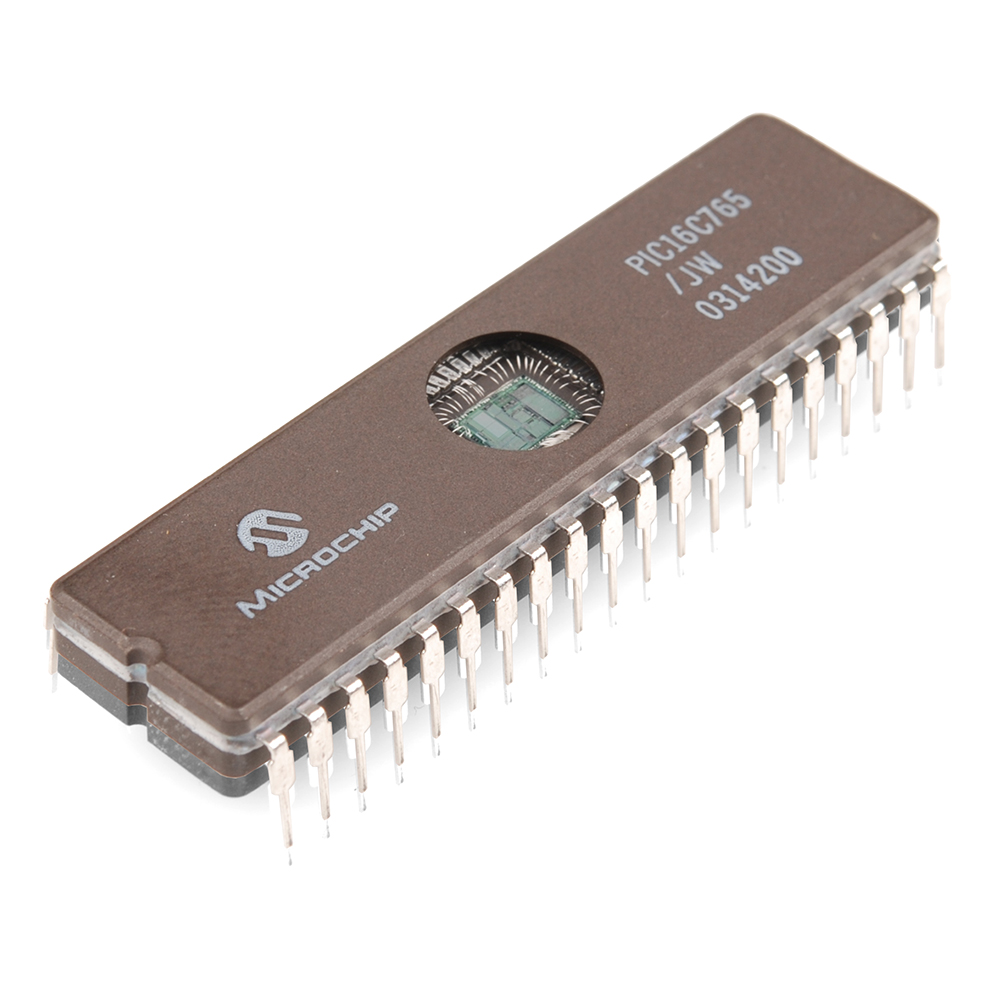
\includegraphics[height=5.2cm, trim=10 31 10 25, clip]{eprom-chip.jpg}% recorte del margen blanco (en bp; la foto mide 240 bp)
    \caption{Microcontrolador PIC16C765/JW: la versión ``JW'' tiene la memoria de programa en EPROM y se reconoce por la ventana.}
  \end{subfigure}\hfill
  \begin{subfigure}[b]{0.48\textwidth}
    \centering
    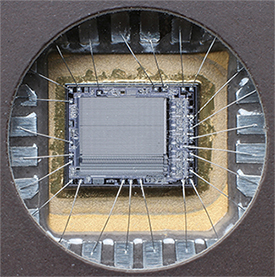
\includegraphics[height=5.2cm]{eprom-ventana.jpg}
    \caption{Detalle de la ventana de cuarzo: a través de ella se ve el chip de silicio y los hilos de conexión.}
  \end{subfigure}
  \caption{EPROM con ventana de cuarzo. Para borrarla se expone el chip a luz ultravioleta a través de la ventana; después se tapa con una etiqueta opaca para que la luz ambiente no la borre de a poco.}
\end{figure}

\subsection{EEPROM (\textit{Electrically Erasable PROM})}

Puede ser \textbf{borrada y reprogramada eléctricamente}, byte a byte, sin necesidad de extraer el chip del circuito. Permite actualizaciones en el propio sistema (\textit{In-System Programming}). Velocidad de escritura más lenta que la RAM; número de ciclos de escritura limitado (típicamente 100.000 a 1.000.000).

\subsection{Memoria Flash}

Es la evolución de la EEPROM. Comparte la capacidad de borrado y escritura eléctrica, pero opera por \textbf{bloques} en lugar de byte a byte, lo que la hace significativamente más rápida en operaciones de borrado. Combina:

\begin{itemize}
  \item Alta densidad de almacenamiento.
  \item No volatilidad.
  \item Lectura/escritura en el propio circuito.
  \item Velocidad de operación comparativamente alta.
  \item Bajo costo por bit.
\end{itemize}

Por estas razones es la tecnología dominante en memorias USB, tarjetas SD y en la \textbf{memoria de programa de los microcontroladores modernos} (incluyendo el ATmega328, que tiene 32 KB de Flash).

\textbf{Comparativa de tipos de ROM:}

\begin{table}[H]
\centering
\begin{tabular}{llll}
\toprule
Tipo & Programación & Borrado & Granularidad borrado \\
\midrule
ROM de máscara & En fábrica & No borrable & --- \\
PROM & Usuario, 1 vez & No borrable & --- \\
EPROM & Usuario & UV, total & Todo el chip \\
EEPROM & Eléctricamente & Eléctricamente & Byte a byte \\
Flash & Eléctricamente & Eléctricamente & Por bloques \\
\bottomrule
\end{tabular}
\end{table}

\section{Expansión de memoria}

En muchas aplicaciones la capacidad o el ancho de palabra de un único chip de memoria no son suficientes. Se pueden combinar varios chips para ampliar la memoria total del sistema. Existen dos técnicas:

\subsection{Expansión de palabra (ampliación de bits por posición)}

Se usa cuando el ancho de palabra de los chips es menor que el del bus de datos del sistema. Los chips se conectan \textbf{en paralelo}, compartiendo el mismo bus de direcciones y las mismas señales de control, pero cada uno aporta algunos bits del bus de datos.

\textbf{Ejemplo:} el bus de datos del sistema es de 8 bits, pero se tienen chips de 4 bits de ancho (organizados como 1K $\times$ 4). Se conectan dos chips en paralelo: uno proporciona D0--D3 y el otro D4--D7. Ambos chips responden a la misma dirección simultáneamente.

\tikzFigura{cap2/expansion-palabra}{Expansión de palabra: dos chips 1K$\times$4 en paralelo forman una memoria 1K$\times$8.}

$$\text{Chips necesarios} = \frac{\text{ancho de palabra del sistema}}{\text{ancho de palabra del chip}}$$

\subsection{Expansión de capacidad (ampliación de direcciones)}

Se usa cuando la cantidad de posiciones de un único chip es menor que la requerida. Los chips se conectan de forma que cada uno responde a un rango diferente de direcciones. Se usa la señal $\overline{CS}$ de cada chip para habilitarlo solo cuando el bus de direcciones está en su rango.

\textbf{Ejemplo:} se necesitan 4K posiciones de 8 bits, pero solo se tienen chips de 1K $\times$ 8. Se conectan 4 chips: el primero responde a las direcciones 0x000--0x3FF, el segundo a 0x400--0x7FF, y así sucesivamente. Un decodificador de 2 a 4 (por ejemplo, el 74139, o un 74138 usando 4 de sus 8 salidas) genera las señales $\overline{CS}$ individuales a partir de las líneas de mayor peso del bus de direcciones.

\tikzFigura{cap2/expansion-capacidad}{Expansión de capacidad: cuatro chips 1K$\times$8 y un decodificador 2 a 4 forman una memoria 4K$\times$8.}

$$\text{Chips necesarios} = \frac{\text{capacidad total requerida}}{\text{capacidad de cada chip}}$$

\subsection{Expansión combinada}

Es posible aplicar ambas técnicas simultáneamente para ampliar tanto el ancho de palabra como la cantidad de posiciones. En ese caso:

$$\text{Chips necesarios} = \frac{\text{capacidad total}}{\text{capacidad del chip}} \times \frac{\text{ancho de palabra del sistema}}{\text{ancho de palabra del chip}}$$
